
%%%%%%%%%%%%%%%%%%%%%%%%%%%%%%%%%%%%%%%%%
% Beamer Presentation
% LaTeX Template
% Version 2.0 (March 8, 2022)
%
% This template originates from:
% https://www.LaTeXTemplates.com
%
% Author:
% Vel (vel@latextemplates.com)
%
% License:
% CC BY-NC-SA 4.0 (https://creativecommons.org/licenses/by-nc-sa/4.0/)
%
%%%%%%%%%%%%%%%%%%%%%%%%%%%%%%%%%%%%%%%%%

%----------------------------------------------------------------------------------------
%	PACKAGES AND OTHER DOCUMENT CONFIGURATIONS
%----------------------------------------------------------------------------------------

\documentclass[11pt]{beamer}

\graphicspath{{images/}{./}}

\usepackage{booktabs}

\usetheme{AnnArbor}
\usecolortheme{seagull}
\usefonttheme{default}

\usepackage{palatino}
\usepackage[default]{opensans} 
\useinnertheme{circles}

%----------------------------------------------------------------------------------------
%	PRESENTATION INFORMATION
%----------------------------------------------------------------------------------------

\title[Razvoj platforme za distribuirano izračunavanje]{Razvoj platforme za distribuirano izračunavanje u oblaku}

\author{Milana Kovačević}

\institute[MATF]{Matematički fakultet, Univerzitet u Beogradu} % Your institution, the optional parameter can be used for the institution shorthand and will appear on the bottom of every slide after author names, while the required parameter is used on the title slide and can include your email address or additional information on separate lines

\date{Master rad \\26. septembar 2022.}

%----------------------------------------------------------------------------------------

\begin{document}

%----------------------------------------------------------------------------------------
%	TITLE SLIDE
%----------------------------------------------------------------------------------------

\begin{frame}
	\titlepage
\end{frame}

%----------------------------------------------------------------------------------------
%	TABLE OF CONTENTS SLIDE
%----------------------------------------------------------------------------------------

\begin{frame}
	\frametitle{Sadržaj}	
	\tableofcontents
\end{frame}

%----------------------------------------------------------------------------------------
%	PRESENTATION BODY SLIDES
%----------------------------------------------------------------------------------------

\section{Uvod}

%------------------------------------------------

\subsection{Distribuirani sistemi}

\begin{frame}
	\frametitle{Distribuirani sistemi}
	
	\begin{block}{Definicija}
		Distribuirani sistemi se sastoje od skupa nezavisnih mašina, koje su medjusobno povezane mrežom. Mašine saradjuju i rasporedjuju poslove kako bi rešile zadati problem.
	\end{block}
	
	\bigskip
	
	Prednosti:
		\begin{itemize}
			\item Visok nivo paralelizacije
			\item Pouzdanost i dostupnost % (izbegavanjem eng. \emph{single point of failure})
			\item Skalabilnost % modularnost
			\item Geo-distribuiranje
		\end{itemize}

	\bigskip

	Mane:
		\begin{itemize}
			\item Oslanjanje na transport poruka kroz mrežu
			\item Složenost
		\end{itemize}

\end{frame}

%------------------------------------------------

\begin{frame}
	\frametitle{Distribuirani sistemi za izračunavanje}

	Sistemi koji se koriste za dostizanje željenih performansi, oslanjajući se na visok stepen paralelizacije.
	
	\bigskip

	Klasteri predstavljaju uvezane čvorove sa podeljenim ulogama - \emph{master} \& \emph{slaves}. Dele lokalnu mrežu i koristete isti operativni sistem.

	\bigskip

	Primeri:
	\begin{itemize}
		\item \emph{Spark}
		\item \emph{Azure Functions}
	\end{itemize}

\end{frame}

%------------------------------------------------

\section{Sistem DCS - \emph{Distributed Computation System}}

\subsection{Motivacija}

\begin{frame}
	\frametitle{Sistem DCS - \emph{Distributed Computation System}}

	\begin{itemize}
		\item Sistem za distribuirano izračunavanje u oblaku
		\item Uspostavljanje zajedničke infrastrukture
		\item Prilagodljivost različitim tipovima poslova
	\end{itemize}

\end{frame}

%------------------------------------------------

\subsection{Funkcionalnosti}

\begin{frame}
	\frametitle{Sistem DCS - Funkcionalnosti}

	\begin{figure}
		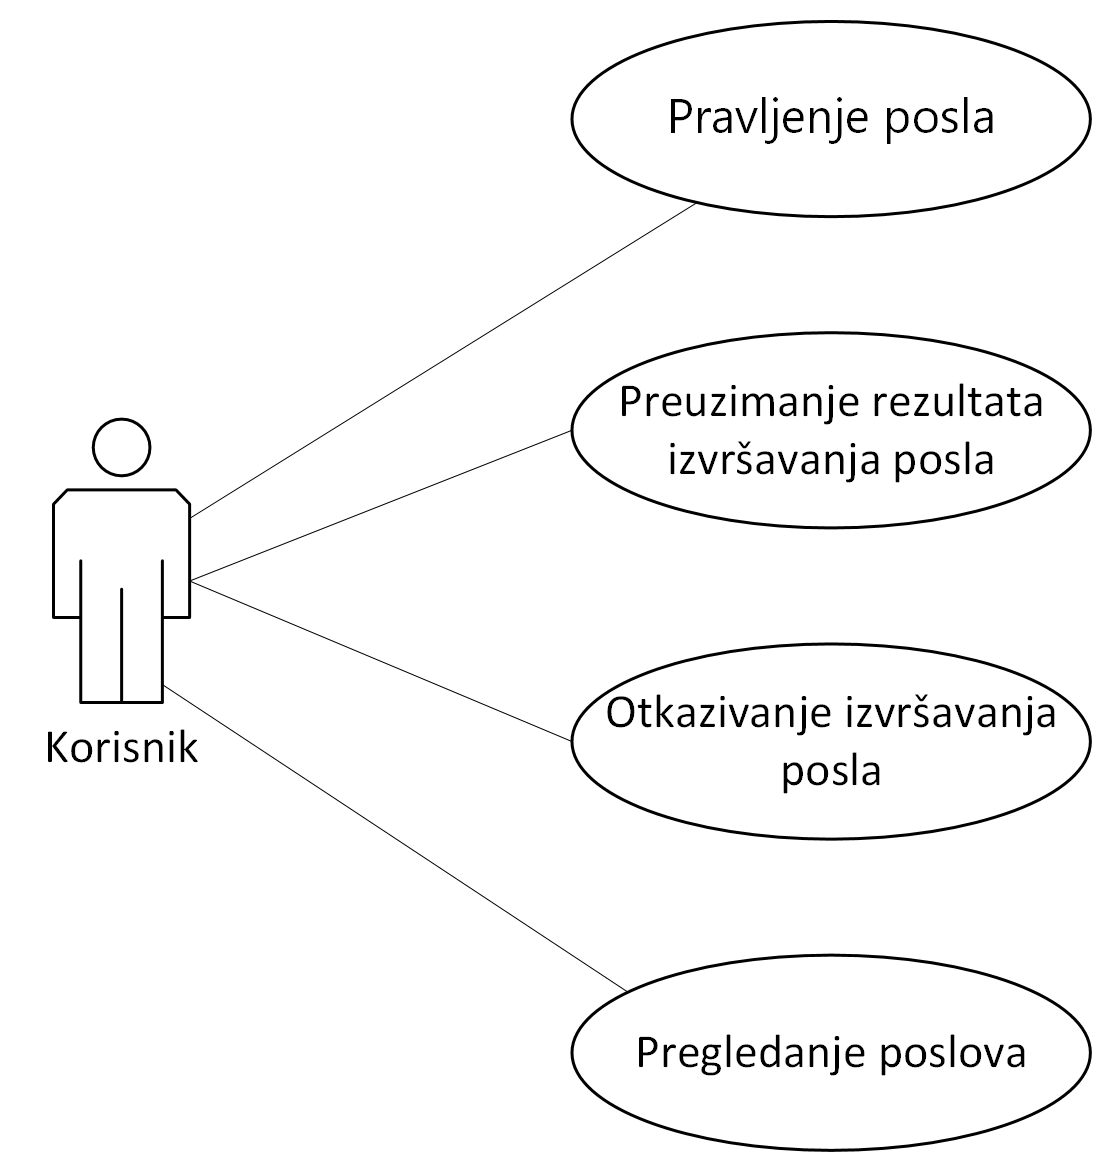
\includegraphics[width=0.55\linewidth]{./images/dijagram_slucajeva_upotrebe_korisnik.png}
	\end{figure}
	
\end{frame}

%------------------------------------------------

\subsection{Implementacija}

\begin{frame}
	\frametitle{Korišćene tehnologije i alati}

	\begin{itemize}
		\item Platforma \emph{Docker}
		\item Platforma \emph{Kubernetes}
		\item Platforma \emph{Microsoft Azure}
		\item \emph{.NET Core}
		\item \emph{Swagger / OpenAPI}
		\item \emph{Dependency injection}
		\item \emph{XUnit}
		\item ...
	\end{itemize}

\end{frame}

%------------------------------------------------


\begin{frame}
	\frametitle{Sistem DCS - Arhitektura}
	
	\begin{figure}
		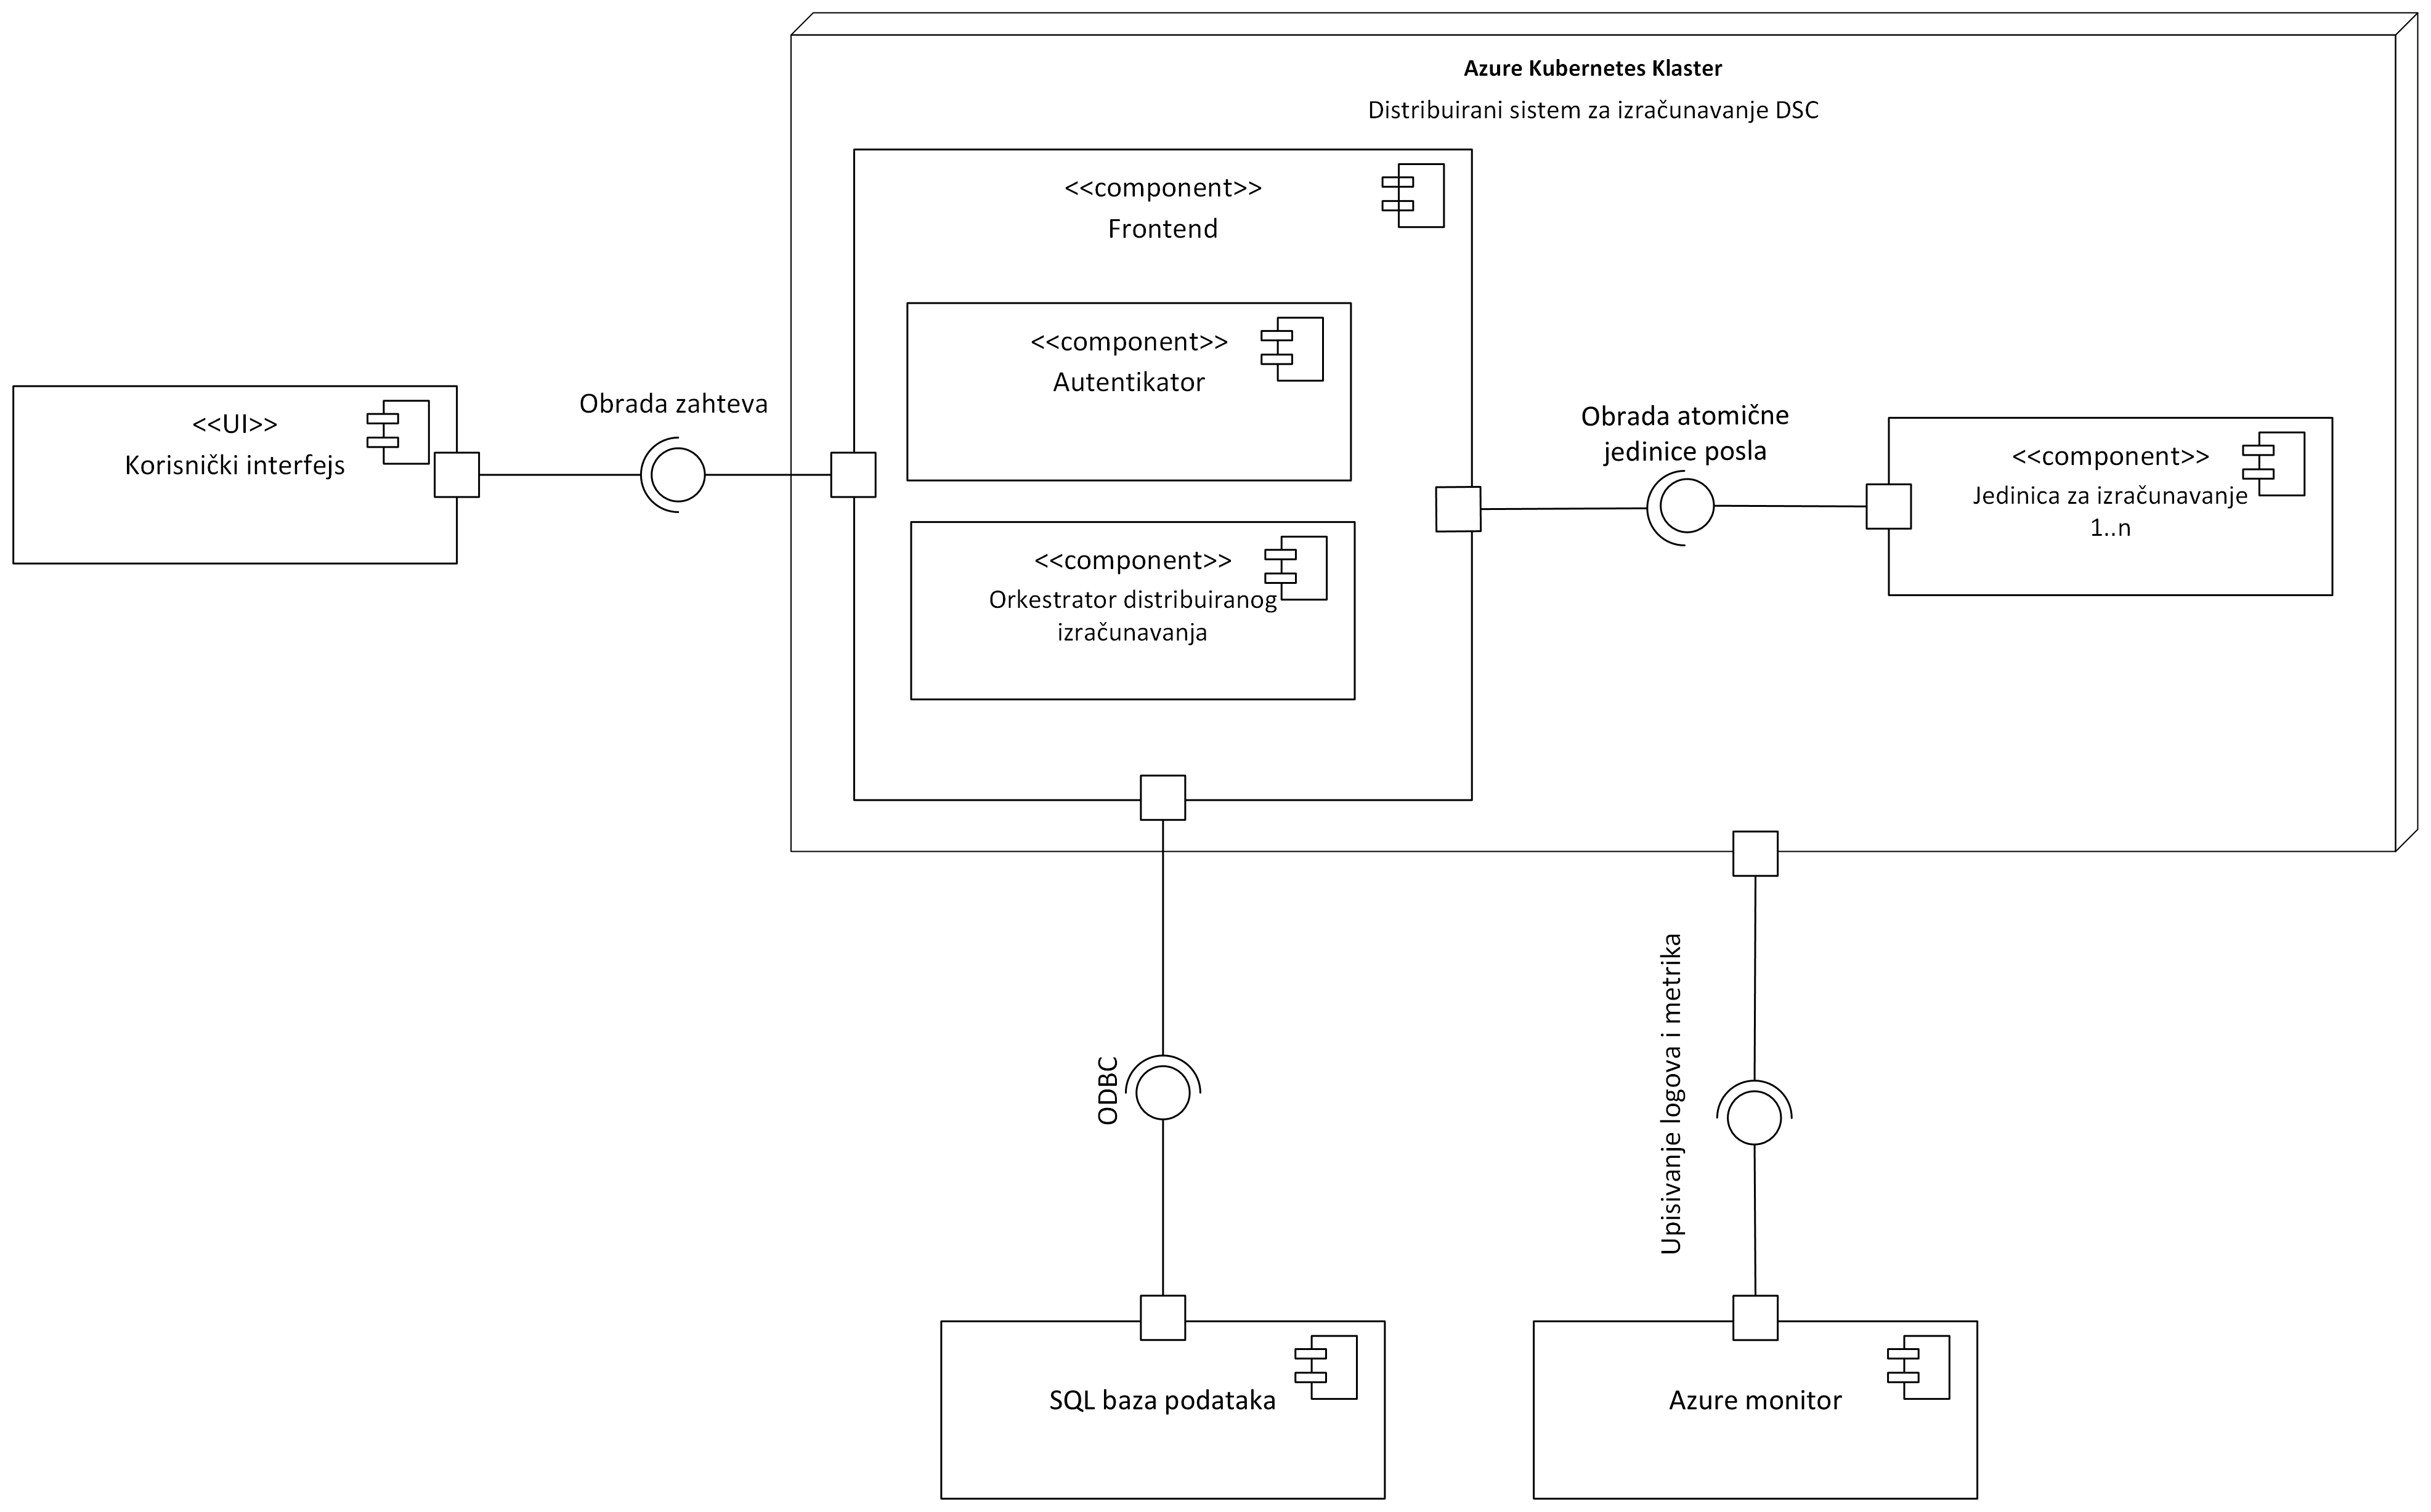
\includegraphics[width=0.9\linewidth]{./images/arhitektura_sistema_dijagram_komponenti.png}
	\end{figure}
\end{frame}

%------------------------------------------------

\begin{frame}
	\frametitle{Demo}

	\begin{center}
		{\Huge DEMO}
	\end{center}

\end{frame}

%------------------------------------------------

\section{Rezultati}

\subsection{Analiza performansi}

\begin{frame}
	\frametitle{Analiza performansi}
	
	\begin{table}
		\begin{tabular}{ll l l l}
			\toprule
			\textbf{Veličina ulaza} & \textbf{sekvencijalno} & \textbf{1 cmpN} & \textbf{5 cmpN} & \textbf{10 cmpN}\\
			\midrule
			 50 & 1.09 & 0.37 & 0.42 & 0.41 \\ 
			 100 & 2.36 & 0.81 & 0.63 & 0.67 \\ 
			 500 & 12.05 & 3.97 & 2.99 & 3.12 \\ 
			 1000 & 23.6 & 8.23 & 6.39 & 6.74 \\ 
			 3000 & 78.16 & 29.17 & 24.12 & 25.84 \\ 
			\bottomrule
		\end{tabular}
		\caption{Prosečno vreme izvršavanja u različitim okruženjima}
	\end{table}

\end{frame}

%------------------------------------------------

\begin{frame}
	\frametitle{Faktor ubrzanja}

	\begin{figure}
		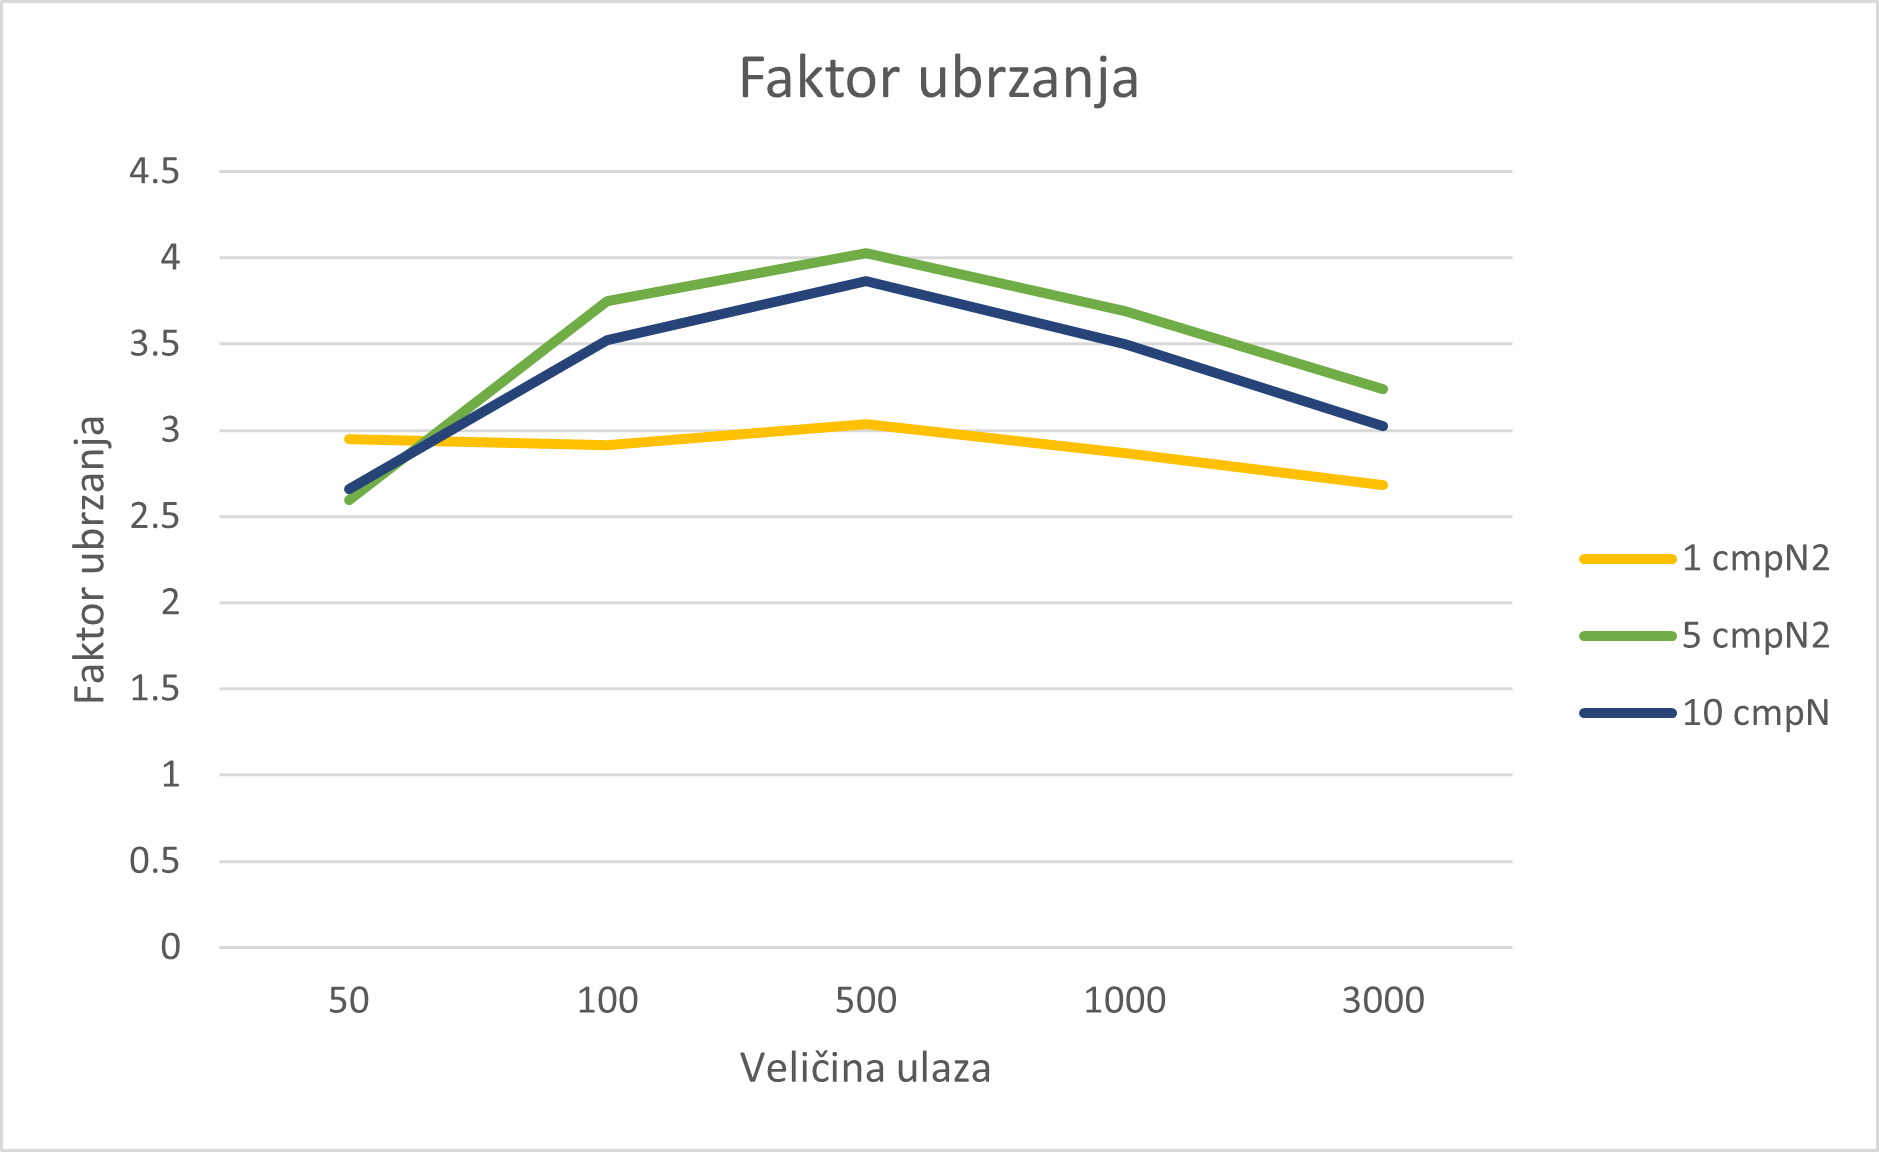
\includegraphics[width=0.9\linewidth]{./images/perf_faktor_ubrzanja.png}
	\end{figure}

\end{frame}

%------------------------------------------------

\subsection{Dalji razvoj sistema}

\begin{frame}
	\frametitle{Dalji razvoj sistema}
	
	\begin{itemize}
		\item Generalizacija tipa poslova
		\item Podrška za različite frontende
		\item Napredno rutiranje zahteva ka jedinicama za izvršavanje
	\end{itemize}

\end{frame}

%------------------------------------------------

\section{Zaključak}

\begin{frame}
	\frametitle{Zaključak}
	
	\begin{enumerate}
		\item Unapredjenje performansi izračunavanja
		\item Modularnost
		\item Skalabilnost
		\item Dalji razvoj definisan prema potrebama korisnika
	\end{enumerate}

\end{frame}

%----------------------------------------------------------------------------------------
%	CLOSING SLIDE
%----------------------------------------------------------------------------------------

\begin{frame}[plain]
	\begin{center}
		{\Huge Kraj}
	\end{center}
\end{frame}

%----------------------------------------------------------------------------------------

\end{document} 